\documentclass[twocolumn]{article}
\usepackage[utf8]{inputenc}
\usepackage{graphicx}
\usepackage{amsmath}
\usepackage{titling}
\usepackage{lipsum}
\usepackage{wrapfig}
\usepackage{romannum}
\usepackage{fancyhdr}
\usepackage[top=2cm, bottom=2cm, left=2cm, right=2cm]{geometry}

\renewcommand{\thesection}{\Roman{section}} 
\renewcommand{\thesubsection}{\thesection.\Roman{subsection}}

\pagestyle{fancy}
\fancyhf{} 
\fancyhead[R]{\today} 
\renewcommand{\headrulewidth}{0pt} 


\fancypagestyle{plain}{ 
    \fancyhf{}
    \fancyhead[R]{\today}
    \renewcommand{\headrulewidth}{0pt} 
}

\title{Physarum polycephalum-Inspired Routing Algorithm for Cave and Catacomb Navigation}

\author{%
    \begin{tabular}{cccc}
        \textbf{Primer Autor} & \textbf{Segundo Autor} & \textbf{Tercer Autor} & \textbf{Cuarto Autor} \\
        \textit{Afiliaci\'on 1} & \textit{Afiliaci\'on 2} & \textit{Afiliaci\'on 3} & \textit{Afiliaci\'on 4} \\
        \texttt{email1@example.com} & \texttt{email2@example.com} & \texttt{email3@example.com} & \texttt{email4@example.com} \\
    \end{tabular}
}

\begin{document}
\maketitle

\begin{abstract}
    El estudio de sistemas biol\'ogicos como el moho del fango Physarum polycephalum, 
        conocido por optimizar rutas de transporte en busca de alimento, inspira el 
        desarrollo de algoritmos de enrutamiento avanzados. Este trabajo introduce 
        un algoritmo de enrutamiento basado en Physarum polycephalum para la navegaci\'on 
        en cuevas y catacumbas. Dise\~nado para mapear entornos subterr\'aneos complejos, 
        el algoritmo utiliza las propiedades de adaptaci\'on y exploraci\'on del moho para 
        determinar rutas \'optimas a trav\'es de laberintos naturales y estructuras subterr\'aneas. 
        Los resultados experimentales indican que el algoritmo mejora la eficiencia en la generaci\'on 
        de caminos y demuestra robustez ante obst\'aculos y variaciones topogr\'aficas, ofreciendo nuevas 
        herramientas para la exploraci\'on arqueol\'ogica y geol\'ogica y avanzando hacia la automatizaci\'on 
        de la exploraci\'on subterr\'anea.
\end{abstract}

\textbf{Keywords—}Physarum polycephalum, routing algorithm, underground navigation, bio-inspired artificial intelligence, cave and catacomb exploration.

\subsubsection{Historia y evoluci\'on}
    \label{subsubsection:historiaEvolucion}
    % Parrafo 1
    La Raspberry Pi naci\'o en 2006 como un proyecto ideado por Eben Upton, Rob Mullins, Jack Lang y Alan Mycroft, 
        quienes trabajaban en la Universidad de Cambridge. La idea principal era crear una computadora de bajo costo 
        que permitiera a los estudiantes de la universidad mejorar sus habilidades de programaci\'on. \cite{Santamaria2023}
        En 2009, el proyecto se convirti\'o en una fundaci\'on sin fines de lucro, la Raspberry Pi Foundation, 
        con el objetivo de promover la ense\~nanza de la inform\'atica en las escuelas y pa\'ises en desarrollo. \cite{Santamaria2023}
    \vskip 0.5cm
    % Parrafo 2
    La primera Raspberry Pi fue lanzada en febrero de 2012, con un procesador ARM11 de 700 MHz, 512 MB de RAM y 
        un precio de 35 d\'olares. Desde entonces, la Raspberry Pi ha evolucionado hasta convertirse en una 
        plataforma de desarrollo muy popular, con millones de unidades vendidas en todo el mundo.\cite{Santamaria2023}
        La Raspberry Pi 4, lanzada en junio de 2019, es la versi\'on m\'as reciente de la placa y cuenta con un 
        procesador ARM Cortex-A72 de 1.5 GHz, hasta 8 GB de RAM y soporte para pantallas 4K. \cite{Santamaria2023}
    \vskip 0.5cm
    % Parrafo 3
    La Raspberry Pi ha sido utilizada en una amplia variedad de proyectos, desde servidores web y centros multimedia 
        hasta robots y sistemas de control. Su bajo costo y su flexibilidad la han convertido en una herramienta 
        muy popular entre los aficionados a la inform\'atica y la electr\'onica. Adem\'as, la Raspberry Pi ha sido 
        utilizada en proyectos educativos en todo el mundo, ayudando a ense\~nar a los j\'ovenes las habilidades 
        necesarias para el siglo XXI.
    \begin{itemize}
        \item \textbf{Raspberry Pi Model B}: La Raspberry Pi Model B es la primera versi\'on de la placa, 
            lanzada en febrero de 2012. Cuenta con un procesador ARM11 de 700 MHz, 512 MB de RAM, 
            1 puerto USB tipo A, 1 conector GPIO de 8 pines, salida HDMI, salida de audio y un lector de tarjetas SD \cite{Santamaria2023}
        \item \textbf{Raspberry Pi Model A+}: La Raspberry Pi Model A+ es una versi\'on m\'as peque\~na y 
            econ\'omica de la placa, lanzada en noviembre de 2014. Cuenta con un procesador ARM11 de 700 MHz, 
            512 MB de RAM, 1 puerto USB tipo A, 1 conector GPIO de 40 pines, salida HDMI y salida de audio 3.5 mm \cite{Santamaria2023}
        \item \textbf{Raspberry Pi 2 Model B}: La Raspberry Pi 2 Model B es la segunda versi\'on de la placa, 
            lanzada en febrero de 2015. Cuenta con un procesador ARM Cortex-A7 de 900 MHz, 1 GB de RAM, 
            4 puertos USB tipo A 2.0, 1 conector GPIO de 40 pines, salida HDMI, salida de audio 3.5mm y ethernet 10/100 \cite{Santamaria2023}
        \item \textbf{Raspberry Pi Zero}: La Raspberry Pi Zero es una versi\'on m\'as peque\~na y econ\'omica 
            de la placa, lanzada en noviembre de 2015. Cuenta con un procesador ARM11 de 1 GHz, 512 MB de RAM, 
            1 puerto mini HDMI, 1 puerto micro USB OTG, 1 conector GPIO de 40 pines y HAT compatible de 40 pines \cite{Santamaria2023} 
        \item \textbf{Raspberry Pi 3 Model B}: La Raspberry Pi 3 Model B es la tercera versi\'on de la placa, 
            lanzada en febrero de 2016. Cuenta con un procesador ARM Cortex-A53 de 1.2 GHz, 1 GB de RAM, 
            4 puertos USB tipo A 2.0, 1 conector GPIO de 40 pines, salida HDMI, salida de audio 3.5mm, ethernet 10/100, 
            conexi\'on Wifi y Bluethooth 4.1 LE \cite{Santamaria2023}
        \item \textbf{Raspberry Pi Zero W}: La Raspberry Pi Zero W es una versi\'on m\'as peque\~na y econ\'omica 
            de la placa, lanzada en febrero de 2017. Cuenta con un procesador ARM11 de 1 GHz, 512 MB de RAM, 
            1 puerto mini HDMI, 1 puerto micro USB OTG, 1 conector GPIO de 40 pines, HAT compatible de 40 pines, 
            conexi\'on Wifi y Bluethooth 4.1 LE \cite{Santamaria2023}
        \item \textbf{Raspberry Pi Zero WH}: La Raspberry Pi Zero WH es una versi\'on m\'as peque\~na y econ\'omica 
            de la placa, lanzada en febrero de 2018. Cuenta con un procesador ARM11 de 1 GHz, 512 MB de RAM, 
            1 puerto mini HDMI, 1 puerto micro USB OTG, 1 conector GPIO de 40 pines, HAT compatible de 40 pines, 
            conexi\'on Wifi y Bluethooth 4.1 LE \cite{Santamaria2023}
        \item \textbf{Raspberry Pi 3 Model B+}: La Raspberry Pi 3 Model B+ es la cuarta versi\'on de la placa,
            lanzada en marzo de 2018. Cuenta con un procesador ARM Cortex-A53 de 1.4 GHz, 1 GB de RAM, 
            4 puertos USB tipo A 2.0, 1 conector GPIO de 40 pines, salida HDMI, salida de audio 3.5mm, ethernet 10/100, 
            conexi\'on Wifi y Bluethooth 4.2 LE \cite{Santamaria2023}
        \item \textbf{Raspberry Pi 3 Model A+}: La Raspberry Pi 3 Model A+ es una versi\'on m\'as peque\~na y 
            econ\'omica de la placa, lanzada en noviembre de 2018. Cuenta con un procesador ARM Cortex-A53 de 1.4 GHz, 
            512 MB de RAM, 1 puerto USB tipo A 2.0, 1 conector GPIO de 40 pines, salida HDMI, salida de audio 3.5mm, 
            conexi\'on Wifi y Bluethooth 4.2 LE \cite{Santamaria2023}
        \item \textbf{Raspberry Pi 4 Model B}: La Raspberry Pi 4 Model B es la quinta versi\'on de la placa,
            lanzada en junio de 2019. Cuenta con un procesador ARM Cortex-A72 de 1.5 GHz, hasta 8 GB de RAM, 
            2 puertos USB tipo A 3.0, 2 puertos USB tipo A 2.0, 1 conector GPIO de 40 pines, 2 salidas micro HDMI, 
            salida de audio 3.5mm, ethernet Gigabit, conexi\'on Wifi y Bluethooth 5.0 LE \cite{Santamaria2023}
        \item \textbf{Raspberry Pi Compute Module 1}: La Raspberry Pi Compute Module 1 es una versi\'on de la placa 
            dise\~nada para su uso en sistemas embebidos, lanzada en abril de 2014. Cuenta con un procesador ARM11 de 700 MHz, 
            512 MB de RAM, 4GB eMMC Flash, Conector SODIMM DDR2 \cite{Santamaria2023}
        \item \textbf{Raspberry Pi Compute Module 3}: La Raspberry Pi Compute Module 3 es una versi\'on de la placa, 
            lanzada en enero de 2017. Cuenta con un procesador BCM2837 de cuatro n\'ucleos a 1.2 GHz, 1 GB de RAM, 4GB eMMC Flash,
            Conector SODIMM DDR2 y Conector GPIO 46 pines \cite{Santamaria2023}
        \item \textbf{Raspberry Pi Compute Module 3 Lite}: La Raspberry Pi Compute Module 3 Lite es una versi\'on de la placa,
            lanzada en enero de 2017. Cuenta con un procesador BCM2837 de cuatro n\'ucleos a 1.2 GHz, 1 GB de RAM,
            Conector SODIMM DDR2 y Conector GPIO 46 pines \cite{Santamaria2023}
        \item \textbf{Raspberry Pi Compute Module 3+}: La Raspberry Pi Compute Module 3+ es una versi\'on de la placa,
            lanzada en enero de 2019. Cuenta con un procesador BCM2837B0 de cuatro n\'ucleos a 1.2 GHz, 1 GB de RAM, 8GB, 16GB y 32 GB eMMC Flash,
            slot MicroSDHC y Conector GPIO 46 pines \cite{Santamaria2023}
        \item \textbf{Raspberry Pi Compute Module 4}: La Raspberry Pi Compute Module 4 es una versi\'on de la placa,
            lanzada en octubre de 2020. Cuenta con un procesador ARM a 1.5 GHz, 1 GB, 2 GB, 4 GB, 8 GB de RAM,
            2 puertos Gigabit Ethernet, Conectividad Wi-Fi (opcional), 1 USB C y conector GPIO de 28 pines \cite{Santamaria2023}
        \item \textbf{Raspberry Pi 400}: La Raspberry Pi 400 es una versi\'on de la placa, lanzada en noviembre de 2020.
            Cuenta con un procesador ARM Cortex-A72 de 1.5 GHz y soporte de 64 bits, 1-8 GB de RAM, 2 puertos USB tipo A 3.0, 2 puertos USB tipo A 2.0,
            Conector GPIO de 40 pines, 2 salidas micro HDMI, salida de audio 3.5mm, ethernet Gigabit, conexi\'on Wifi y Bluethooth 5.0 LE \cite{Santamaria2023}
        \item \textbf{Raspberry Pi Pico}: La Raspberry Pi Pico es una placa de desarrollo, lanzada en enero de 2021.
            Cuenta con un procesador RP2040 de doble n\'ucleo ARM Cortex-M0+ a 133 MHz, 264 KB de RAM, 2 MB de memoria flash QSPI,
            26 pines GPIO, 3 pines anal\'ogicos, 2 UART, 2 SPI, 2 I2C, 16 canales PWM, 1 temporizador de 12 bits y 1 temporizador de 16 bits \cite{Santamaria2023}
        \item \textbf{Raspberry Pi Zero 2 W}: La Raspberry Pi Zero 2 W es una versi\'on de la placa, lanzada en octubre de 2021.
            Cuenta con un procesador BCM2710A1 de cuatro n\'ucleos a 1.0 GHz, 512 MB de RAM, 1 puerto mini HDMI, 1 puerto micro USB OTG, 1 conector GPIO de 40 pines, HAT compatible de 40 pines,
            conexi\'on Wifi y Bluethooth 4.2 LE \cite{Santamaria2023}
        \item \textbf{Raspberry Pi 5}: La Raspberry Pi 5 es una versi\'on de la placa, lanzada en octubre de 2023. 
            Cuenta con un procesador ARM Cortex-A73 de 2.4 GHz, hasta 8 GB de RAM, Doble salida micro HDMI 4K60p, gpu VideoCore VII con soporte 
            de OpenGL ES 2.1 y Vulkan 1.2, decodificador HEVC 4K60, Bluethooth 5.0, WiFi 802.11ac, Ranura microSD de alta velocidad con soporte de SDR104, 
            2 puertos USB 3.0, 2 puertos USB 2.0, 1 puerto Gigabit Ethernet, interfaz PCIe 2.0, conexiones GPIO de 40 pines y bot\'on de encendido y apagado \cite{Santamaria2023}
    \end{itemize}
    

\subsubsection{Physarum Polycephalum}
\label{ssub:PhysarumPolycephalum01}
    %Parrafo 1
    El Physarum Polycephalum, tambi\'en conocido como "The Blob", 
        o "La Mancha", es un protista con formas celulares diversas. El Physarum Polycephalum
        es un mixomiceto acelular, esto proviene de la etapa plasmoidal de su ciclo de vida,
        en la cual el plasmodio es un coenocito multinucleado macroscopico de color amarillo 
        brillante, formado en una red de tubos entrelazados. Esta etapa del ciclo de vida es 
        la que se utiliza para el estudio de este organismo.\cite{Dee1960} Podemos ver un ejemplo
        en la siguiente Figura \ref{fig:PhysarumPolycephalum01}.
    \begin{figure}[h]  
        \centering
        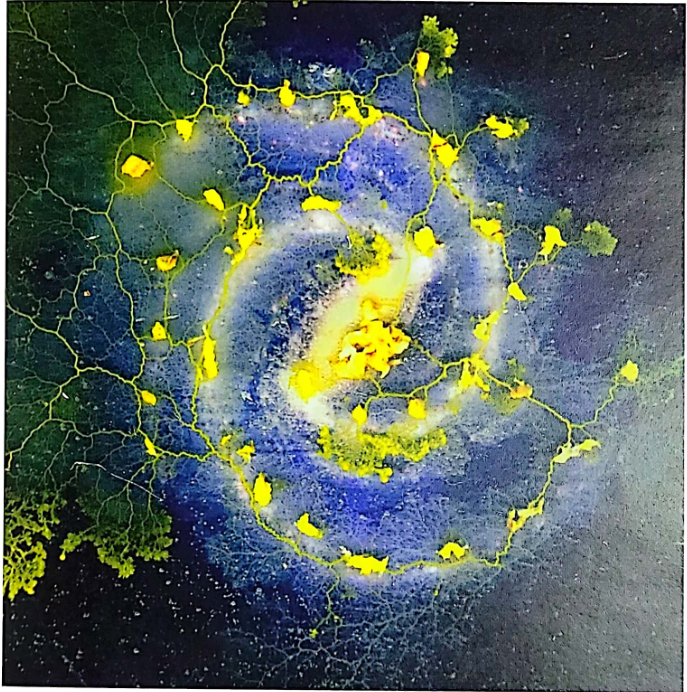
\includegraphics[width=0.5\textwidth]{./images/marco_teorico/Physarum/PhyrasumPolycephalum01.png}
        \caption{Physarum propag\'andose en una impresi\'on art\'istica de una galaxia. Imagen extra\'ida de 'Atlas of Physarum Computing' de A. Adamatzky \cite{Adamatzky2014}.}
        \label{fig:PhysarumPolycephalum01}
    \end{figure} 
    \vskip 0.5cm
    %Parrafo 2
    Como vimos con anterioridad, los mixomicetos se dividen en dos etapas, el plasmodio y los cuerpos fruct\'iferos.
        El Physarum Polycephalum es un mixomiceto que se encuentra en la etapa plasmodial de su ciclo de vida, 
        en la cual el plasmodio es un coenocito multinucleado macroscopico de color amarillo brillante, formado en una red de tubos entrelazados.
        Esta etapa del ciclo de vida es la que se utiliza para el estudio de este organismo.\cite{Dee1960}
    \begin{wrapfigure}{r}{0.17\textwidth}
        \centering
        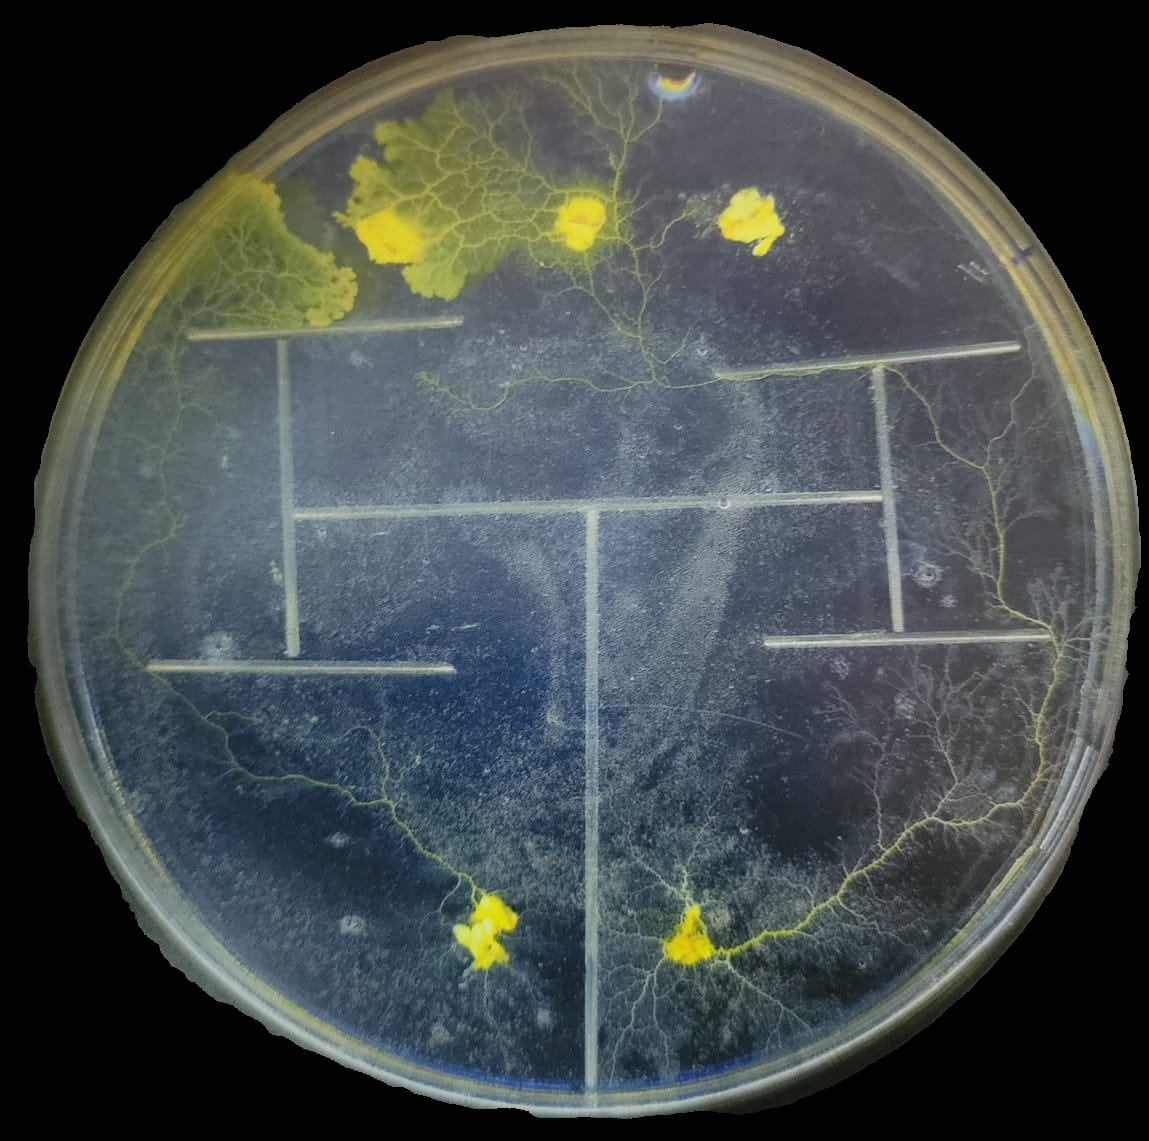
\includegraphics[width=0.17\textwidth]{./images/marco_teorico/Physarum/LaberintoPhysarum.png}
        \caption{Physarum Polycephalum resolviendo un laberinto. \cite{Adamatzky2014}.}
        \label{fig:PhysarumPolycephalum02}
    \end{wrapfigure}
    \vskip 0.5cm
    %Parrafo 3
    El Physarum Polycephalum es un organismo que se encuentra en la naturaleza en lugares h\'umedos y oscuros, 
        como en el interior de los troncos de los \'arboles en descomposici\'on, en hojarasca h\'umeda, en suelos 
        ricos en materia org\'anica y en lugares oscuros y h\'umedos. Este organismo se alimenta de bacterias, 
        hongos y otros microorganismos que se encuentran en su entorno, y se desplaza por medio de la contracci\'on 
        de sus fibras de actina, que le permiten moverse en busca de alimento.\cite{Dee1960}
    \vskip 0.5cm
    %Parrafo 4
    El Physarum Polycephalum es un organismo muy interesante para el estudio de la biolog\'ia y la f\'isica, 
        ya que tiene propiedades \'unicas que lo hacen un organismo muy especial. Por ejemplo, el Physarum Polycephalum 
        es capaz de resolver laberintos como se observa en la Figura \ref{fig:PhysarumPolycephalum02}, encontrar la ruta m\'as corta entre dos puntos, y tomar decisiones complejas 
        basadas en la informaci\'on que recibe de su entorno. Adem\'as, el Physarum Polycephalum es capaz de aprender 
        y recordar informaci\'on, y de adaptarse a su entorno de una manera muy eficiente.
    \vskip 0.5cm
    %Parrafo 5
    Una vez dada una breve introducci\'on al Physarum Polycephalum, podemos pasar a la perspectiva de la computaci\'on, 
        en donde el Physarum Polycephalum ha sido utilizado para resolver problemas de optimizaci\'on, simulaci\'on 
        de redes de transporte, y modelado de sistemas complejos. En la siguiente secci\'on veremos c\'omo el Physarum 
        Polycephalum ha sido utilizado en la computaci\'on y en la modelaci\'on de sistemas complejos.
    

\section{Desarrollo}
\lipsum[6-10]

\subsection{Otro Tema}
\lipsum[11]

\section{Conclusiones}
\lipsum[12]

\begin{thebibliography}{00}
\bibitem{b1} Referencia del primer elemento.
\bibitem{b2} Referencia del segundo elemento.
\end{thebibliography}

\end{document}
